%        File: WeeklyResearchReport_4_19_21.tex
%     Created: Mon Apr 19 08:00 AM 2021 E
% Last Change: Mon Apr 19 08:00 AM 2021 E
%
\documentclass[a4paper]{article}
\usepackage{mathtools}
\usepackage{verbatim}
\usepackage{graphicx}
\usepackage{tabularx}
\usepackage{pgfplots}
\usepackage{adjustbox}
\usepackage{booktabs}
\makeatletter
\let\latex@xfloat=\@xfloat
\def\@xfloat #1[#2]{%
    \latex@xfloat #1[#2]%
    \def\baselinestretch{1}
    \@normalsize\normalsize
    \normalsize
}
\makeatother
\usepackage{amsmath}
\usepackage{mathtools}
\usepackage{epigraph}
\usepackage{cancel}
\usepackage{xcolor}
\newcommand\Ccancel[2][black]{\renewcommand\CancelColor{\color{#1}}\cancel{#2}}
\usepackage{algorithm}
\usepackage{graphicx}
\usepackage[noend]{algpseudocode}
\usepackage{gnuplot-lua-tikz}
\usepackage[utf8]{inputenc}
\usepackage{pgfplots}
\usepackage{tabularx}
\DeclareUnicodeCharacter{2212}{−}
\usepgfplotslibrary{groupplots,dateplot}
\usetikzlibrary{patterns,shapes.arrows}
\pgfplotsset{compat=newest}
\begin{document}
\begin{titlepage}

    \title{
    Daily Research Report}

    \author{ Jeffrey Severino \\
        University of Toledo \\
        Toledo, OH  43606 \\
    email: jseveri@rockets.utoledo.edu}


    \maketitle

\end{titlepage}
\section{Current Research Direction}
I have been writing my own version of a results section that is checking Kousens
work. I am starting with the analytical solution and I have confirmed that my 
notes confirm Kousens equation 4.1. by checking Kerrebrocks ``Aircraft Engines 
and Gas Turbines, 2nd Edition'' Chapter 9, section 9.3 which was very succinct 
and included a nice sanity check. 
\section{Research Performed}
\begin{itemize}
    \item Drafted analytical solution documentation started reviewing the draft.
    \item Started coding up the analytical solution shown in Kerrebrock's book. 
        Kousen cited Shakar's references. The analytical solution should 
        provide a way to check the eigenvalues and vectors.
\end{itemize}
\begin{figure}[h!]
    \centering
     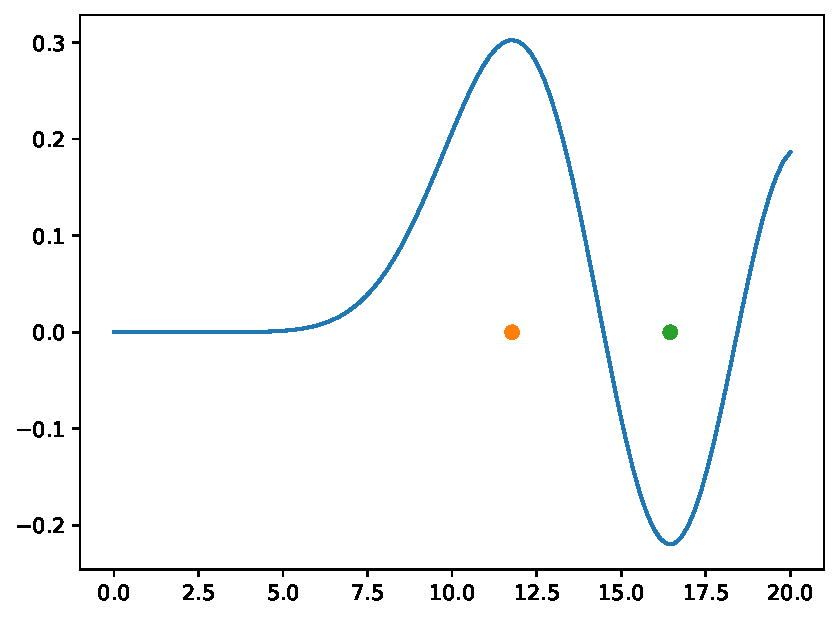
\includegraphics[width=\textwidth]{/home/jeff-severino/SWIRL/CodeRun/03-plotReport/tex-outputs/bessel_mode.pdf}
    \caption{Bessel Mode shown in kerrebrock and the derivative zeros needed for solution }
\end{figure}<++>
\section{Issues and concerns}
I have two ways of obtaining the zero crossings for the analytical solution. The
simplest way is to use Python's Scipy library, however, the infrastructure for
using the intrinsics in FORTRAN has been coded and Python and can be used as 
psudocode for a faster FORTRAN 90 code.
\section{Planned Research}
Include sanity checks in the AnalyticalDuctModes.pdf that show the level of detail as 
shown in Kerrebrock.
\end{document}


